\section{提案システム}
%第\ref{sec:related-works}で述べたように,これまでに提案されてきた検知に基づくDNS Tunneling対策には,Low Throughput手法および転送頻度を下げる手法に対して,検知が困難であるという課題がある.
%他方,新しいアーキテクチャに基づく名前解決システムには,マイグレーションの課題が残留している.
本章では,提案システムについて説明する.
はじめにシステムの概要と目的を示す.
次に,システムの詳細に関して,アーキテクチャ・動作メカニズム・プロトコル・スケーラビリティを順に説明する.

\subsection{Tunneling抑止指向型名前解決システム : SORES}
本節では,システムの概要について説明する.

SORES(Symbol Oriented Records rEsolution System)は,全てのレコード情報をシンボルとなる識別子が付与し,フラットな名前空間で管理することによって,問い合わせの際にシンボル指向でレコード情報を解決する名前解決システムである.
シンボルには,224bitの名前空間をもつハッシュ関数によって算出されるメッセージダイジェストを使用する.
具体的なレコード情報は,ゾーンを管理するサーバノードに階層的に連結したノードのよって作成・更新・破棄される.
SORESの名前空間は,ソートされたハッシュ値の範囲に基づき分割され,既存システムのTLDによって分割された範囲をゾーンとして分割的に管理される.
SORESにおけるクライアントは,シンボルを算出することによって,レコード情報を保持するノードを一意に特定することができる.
また,シンボルからレコード情報を保持するノードを一意に特定の名前解決プロセスでは,レコード情報を作成したエンティティは介在されない.
すなわち,レコード情報を作成する機能とレコード情報を管理する機能を異なるサービスノードに分離させることによって,SORESではDNS Exfiltrationが発生することを抑止する.

SORESでは,DNS Infiltrationに対して,認証基盤の導入と使用できるリソースレコードを制限するメソッドを採用する.
認証基盤では,ドメインに関連づけるレコード情報との関連性を評価することで不審なレコード情報がハッシュテーブル上にストアされることを防止する.
QNAMEにシンボルとして224bitのメッセージダイジェストを使用することによって,副次的効果として,偽装DNS応答パケットの作成が困難にできるという性質が期待される.
また,既存システムにおけるDNSSECによって実現されてきた送信元のトレーサビリティについて,SORESでは認証基盤とシンボルに基づくDNS応答パケットの偽装困難性によって実現され,DNSSECの必要性はなくなる.
さらに,任意の文字列を注入することができるレコードタイプ``NULL"と``TXT"について,実験目的のNULLタイプの使用制限とTXTタイプは機能をシンタックスの限定しているSPFに回帰させることで対処する.

SORESの特徴を以下に示す.
\begin{itemize}
 \item シンボルに基づく名前解決システム
 \vspace{-3mm}
 \item フラットな名前空間
 \vspace{-3mm}
 \item ソートされた範囲に基づくゾーン分割
 \vspace{-3mm}
 \item レコード情報の操作機能と管理機能の分離
 \vspace{-3mm}
 \item 認証されたレコード情報
\end{itemize}

\begin{figure}[t]
 \centering
 \label{fig:abstruct-SORES-architecture}
 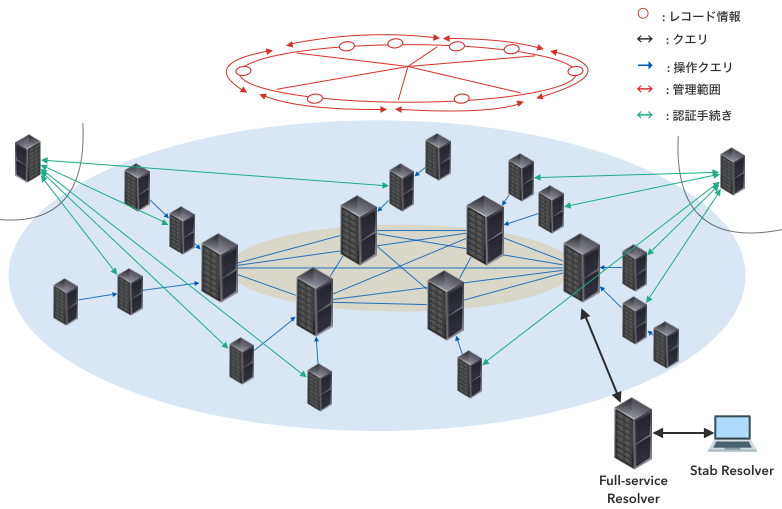
\includegraphics[scale=0.5]{figure/abstruct-architecture.png}
 \caption{SORESの全体図}
\end{figure}


\subsection{デザイン}
\subsubsection{P2Pを組み合わせたハイブリッドなアーキテクチャ}

\begin{figure}[bh]
 \centering
 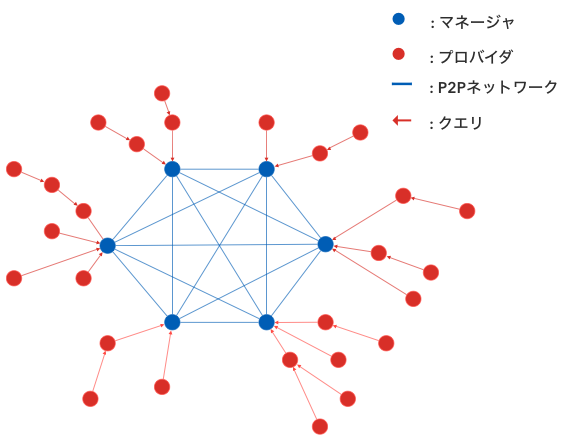
\includegraphics[scale=0.5]{figure/manager-provider.png}
 \caption{マネージャとプロバイダの関係図}
 \label{fig:manager-provider}
\end{figure}

全体のアーキテクチャに関して,SORESでは,既存のDNS同様にクライアントサーバアーキテクチャで構成される.
サーバは,フルメッシュネットワークで相互に接続される固定ノードによるP2Pネットワークアーキテクチャで構成される.

SORESにおけるサービスノードは,機能に基づいて4つに分けることができる.
スタブリゾルバは,既存のDNSと同様に動作するノードであり,DNSクライアントとして名前解決を依頼する主体として位置づくノードである.
フルサービスリゾルバもスタブリゾルバ同様,1つ追加機能を除いて変更点はなく,スタブリゾルバからの問い合わせに対してリソース情報を保持する主体に代理的に問い合わせ機能と,問い合わせた情報を一定期間キャッシュするキャッシュサーバとして機能するノードである.
変更された点は,以降で説明するように,SORESではレコード情報に対する識別子をキーとしてアクセスする.
フルサービスリゾルバは,スタブリゾルバからの従来のフォーマットのDNSクエリについて,ドメイン名とレコードタイプからハッシュ値の算出を行う機能を担う.
算出したハッシュ値をキーとして,フルサービスリゾルバは,サーバに転送する.
SORESでは,権威サーバが機能に基づき二つサービスノードに分割される.


マネージャは,実際のレコード情報を保持し,クライアントからの問い合わせに応答するサーバノードである.
また,マネージャは,既存のDNSにおけるTLDに位置づく権威サーバが担当する.
続いて,4つ目のサービスノードとなるプロバイダは,レコード情報を作成・更新および消去といった操作を担当する.
プロバイダは,既存のDNSにおけるSLD以降の権威サーバに相当し,ドメインの階層構造を従いマネージャに接続される.
プロバイダは,マネージャを介在することで,レコード情報を操作することができる.
例えば,example.comプロバイダが``www"のIPアドレス情報を作成することを考える.
example.comプロバイダは,``www.example.com"とレコードタイプ``A"およびその値``93.184.216.34"を含むデータを接続先のcomマネージャにリクエストする.
comマネージャは,リクエストされたドメイン名とそれに関連づけるレコードタイプから識別子を算出し,担当のマネージャにストアリクエストを転送するという具合で動作する.
SORESにおける用語については,表~\ref{tab:refres-terminology}で示す.
\begin{table}[h]
 \centering
  \begin{tabular}{cl}
    \toprule
    \multicolumn{1}{c}{\textbf{表記}} & \multicolumn{1}{c}{\textbf{意味もしくは機能}}\\
    \midrule

    コンテンツ & \begin{tabular}{l}・識別子に関連づけられたレコード情報の実体\end{tabular}\\ \hline

    コンテンツID & \begin{tabular}{l}・識別子\end{tabular}\\ \hline

    レコード情報 &
      \begin{tabular}{l}
        ・リソースレコードの具体的な値\\
        (E.g. IPアドレス)
      \end{tabular}\\ \hline

     リソースレコードタイプ &
      \begin{tabular}{l}
        ・オブジェクトに関連づけるリソースレコードの型\\
        (E.g. A, AAAA, MX)
      \end{tabular}\\ \hline

    オブジェクト &
      \begin{tabular}{l}
       ・問い合わせる対象\\
       (E.g. ドメイン名もしくはIPアドレス)
      \end{tabular}\\ \hline

    スタブリゾル & \begin{tabular}{l}・名前解決クライアント\end{tabular}\\ \hline

    フルサービスリゾルバ &
      \begin{tabular}{l}
       ・スタブリゾルバからのクエリハンドリング\\
       ・識別子の作成
      \end{tabular}\\ \hline

    マネージャ &
      \begin{tabular}{l}
       ・フルサービスリゾルバからのクエリハンドリング\\
       ・ゾーンの管理\\
       ・コンテンツの保持
      \end{tabular}\\ \hline

    プロバイダ & \begin{tabular}{l}・コンテンツの作成・更新・削除操作\end{tabular}\\

    \bottomrule
  \end{tabular}
 \label{tab:refres-terminology}
 \caption{SORESにおける用語}
\end{table}


\subsubsection{識別子と名前空間}
本項では,レコード情報にアクセスするために用いる識別子,コンテンツIDとその名前空間について説明する.
既存のDNSの名前解決システムでは,正引きをする際,ドメイン名とレコードタイプの二つの情報をキーとして,サーバは保持するゾーンファイルから該当するレコード情報が求まる.
他方,SORESでは,ドメイン名とレコードタイプに基づき算出されるコンテンツIDを識別子として指定することでレコード情報にアクセスする.

におけるレコード情報へのアクセス方法は,識別子をキーとすることでデータを取得することができる.
コンテンツIDと呼ぶ,この識別子は,ドメイン名とレコードタイプの順番でその文字列の和を引数とするメッセージダイジェストで表現することができる.
例えば,ドメイン名を``www.example.com",レコードタイプを``A"とした場合,引数となるのは``www.example.comA"という具合である.
%以上のことから,224bitの名前空間をSORESでは採用する.
% 224bitの名前空間を持つこととダイジェストの長さは違う
% sha3_224のダイジェスト長は,56文字

続いて,SORESが採用するハッシュアルゴリズムについて説明する.
SORESでは,全てのコンテンツIDがフラットな名前空間上にマップされる.
従来では,異なるリソースレコードタイプのレコード情報について一つのゾーンファイルに記述することで,管理することができた.
他方で,SORESでは,ドメイン名とリソースレコードタイプの組をハッシュ値の引数とするため,コンテンツIDは,レコード情報の数に比例して増加する特性がある.
また,識別子の引数の一つにドメイン名が含まれていることから,識別子から元のメッセージが導き出くことが困難な性質を備えていなくてはならない.
この性質を満たすことで,なんらかの方法で識別子を悪意の第三者が取得した際にDNS Exfiltrationとして機能してしまうことを抑止することができる.
最後に,SORESでは,既存のDNSのプロトコルフォーマットを流用する設計になっているため,識別子が格納されるDNSのQuestion SectionのQNAMEのサイズ制約を満たさなくてはならない.
QNAMEは,最大253byteとする任意長の領域である.
以上のことを踏まえて,本システムにおけるハッシュアルゴリズムの要件は,以下の通りである.

\begin{enumerate}
 \item 名前空間は不足を無視できる程度に大きくなくてはならない
 \vspace{-3mm}
 \item アルゴリズムは一方向性の性質を備えなくてはならない
 \vspace{-3mm}
 \item 最大253byteの出力長を満たさなくてはならない
 \vspace{-3mm}
\end{enumerate}

ここで,既存のハッシュ関数の特性をまとめたtableを示す.

上記の内容から,SORESでは,224bitの名前空間をもつsha3のアルゴリズムを採用する.

続いて,分離連鎖法と2重ハッシュ法によるコリジョン対策方法について説明する.
SORESでは,コンテンツのストアリングフェーズでIDにコリジョンが発生した場合,分離連鎖法に基づきストアされるハッシュテーブルに連結リストという形式でコンテンツがストアされる.
リスト構造で延長するコンテンツの識別には,ドメインIDを識別子として利用する.
ドメインIDは,コンテンツIDと同様のハッシュアルゴリズムを用いて算出されるメッセージダイジェストの先頭32bitで表現される,ドメイン名を引数として生成される識別子である.
例えば,ドメイン名を``www.example.com"とする場合,そのメッセージダイジェストが``86ff20100c058b857bae9785bf0267e6c6afb740c18b8e9a87258485"であるとすると,``86ff"がドメインIDとなる具合である.
このように算出されたドメインIDは,DNSのQuestion Sectionのうち,それぞれ16bit分の領域を持つタイプとクラスの領域に埋め込まれる.
上記の仕組みによって,コリジョンが発生した際には,ドメインIDをキーとしてコンテンツを識別する.


\subsubsection{ソートされたハッシュ空間の範囲に基づいたゾーン}
本項では,ゾーンの分割方法およびマネージャノードのアドレスとそのゾーンの範囲に関する対応表について説明する.
はじめに比較のために,従来のシステムの場合について説明する.
従来のシステムでは,ドメインの階層構造に従い,ドメインの管理ノードを下位のドメイン管理ノードに委譲することでゾーンが分割される.
この仕組みでは,ゾーン内の全てのレコード情報はゾーンファイルに画一的にまとめられ,そのゾーンを管理する権威サーバがレコード情報の保持機能とクライアントから応答するという二つの機能を担う.
このゾーン分割メソッドでは,レコード情報の帰属が明確であり,ドメインの管理ノードがトラストアンカーとしての役割を同時に担うことができるメリットがある.
一方のSORESでは,識別子を算出する際に使用するハッシュ関数によって構成される名前空間に基づき,ソートされたハッシュの名前空間の連続した範囲で分割する.
この分割された連続した範囲に基づきゾーンがマネージャに割り当てられることで,既存システム同様にレコード情報全体を分散的に管理する.

上記で説明するように,マネージャが管理するゾーンは,ハッシュの名前空間の連続した一部の範囲である.
従って,レコード情報は,ハッシュの名前空間上で識別子をソートした際に,帰属する範囲を管理するマネージャによって保持される.
マネージャのアドレスを解決する方法には,ゾーンとしてハッシュ値の範囲とそのマネージャおよびマネージャのアドレスに関する対応表~\ref{tab:hash-management}によって解決される.
SORESでは,全てのサービスノードがこの対応表を保持できることを想定しており,ノードは識別子に基づきどのマネージャがコンテンツを保持しているのかを一意に特定する.
\begin{table}[htb]
 \caption[マネージャとゾーンの対応表]{マネージャの情報とそのマネージャが管理するゾーンが記載された対応表の例}
 \centering
  \begin{tabular}{lrl}
    \toprule
		\multicolumn{1}{c}{\textbf{ゾーン}} & \begin{tabular}{c}\textbf{マネージャ}\\\textbf{アドレス}\end{tabular} & \multicolumn{1}{c}{\textbf{ドメイン}} \\
    \midrule
    (000…00, 2zz…zz) & 192.35.51.30 & com.  \\
		\multicolumn{1}{c}{...} & \multicolumn{1}{c}{...} & ... \\
    (500…00, 6zz…zz) & 192.5.6.30 & net. \\
		\multicolumn{1}{c}{...} & \multicolumn{1}{c}{...} & ... \\
    (b00…00, czz…zz) & 199.249.112.1 & org. \\
		\multicolumn{1}{c}{...} & \multicolumn{1}{c}{...} & ... \\
    (n00…00, mzz…zz) & 199.254.31.1 & info. \\
		\multicolumn{1}{c}{...} & \multicolumn{1}{c}{...} & ... \\
    (y00…00, zzz…zz) & 194.0.0.53 & arpa. \\
    \bottomrule
  \end{tabular}
 \label{tab:hash-management}
\end{table}


\subsubsection{認証基盤に基づく信頼されるレコード情報}
\label{sec:certificate}
% 認証局を導入するとインターネットの匿名性を実現することが難しくなるのではないか
% レコード情報に認証局を導入する場合,webなどのサービスやコンテンツを提供するのが少し困難になるではないかという懸念
% githubなどにおいては,同一ドメインにファイルという形でユーザにディスクを提供している
% CAを委譲する仕組みがある.これによって,
本項では,レコード情報の信頼性担保のための認証基盤について説明する.
\begin{figure}[h]
 \centering
 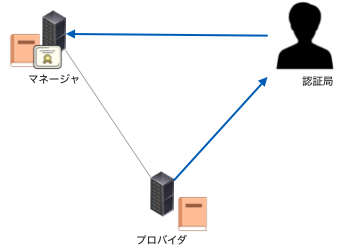
\includegraphics[scale=0.5]{figure/certificate-procedure.png}
 \caption{レコード情報に対する認証プロセス}
 \label{fig:manager-provider}
\end{figure}

SORESでは,全てのコンテンツについて,信頼される第三者からストアしても良いと認可されていることを前提としている.
すなわち,ハッシュテーブル上のコンテンツへの操作,またはコンテンツをハッシュテーブル上にストアするなどの操作処理をする際,プロバイダは,信頼される第三者からのレコード情報に操作することを認可してもらう必要がある.
認可の証明書を発行する認証局は,プロバイダの基本情報とレコード情報に基づき証明書の発行を決定する.
いま,ドメイン名``www.example.com"のリソースレコードタイプAとして``93.184.216.34"というレコード情報を関連づけるとする.
プロバイダは,認証局に対して証明書発行リクエストを転送する.
認証局は,リクエストされたレコード情報についてIPアドレスの到達性と不審な文字列が含まれていないこと,利用目的について評価を施す.
認可された場合には,その証にディジタル証明書を発行し,マネージャにストアリクエストを転送する.
マネージャは,ディジタル証明書に付与された署名に基づきコンテンツの完全性を評価し,認証された場合コンテンツIDを計算し,担当マネージャにストアリクエストを転送する.
上記の手続きを経たコンテンツがハッシュテーブル上にストアされる.


\subsubsection{リソースレコードタイプの選別によるDNS Infiltration対策}
本項では,SORESで使用するリソースレコードのタイプについて説明する.

はじめに,SORESにおけるDNSSECの位置づけについて述べる.
DNSSEC~\cite{rfc4033}は,権威サーバからの応答パケットの偽装を検知することを目的として,データの作成元の確認とデータの完全性および,不在情報応答情報の証明するDNSの拡張仕様である.
これは,主としてDNSの応答パケットを偽装できる程度のパラメータであることに起因する.
他方で,SORESでは,応答パケットに224bitのメッセージダイジェストが含まれるため,悪意のある応答パケットをフルサービスリゾルバに意図的にキャッシュすることは極めて困難である.以上の理由から,SORESではDNSSECの目的にそぐわないため,リソースレコードとして使用されない.

次に,DNSSEC以外のリソースレコードについて説明する.
第~\ref{sec:dns-infiltration}項で示すように,既存の名前解決システムでドメインに関連づけることができるリソースレコードのいくつかのタイプは,DNS Infiltrationとして機能することができる.
DNS Infiltrationを抑止するリソースレコードであることの必要条件は,ドメインに関連のない任意の文字列がレコード情報に含められないことである.
既存のDNSのリソースレコードのタイプのうち,任意の文字列を含めることができるのタイプは以下の通りである.

\begin{table}[htb]
 \centering
  \begin{tabular}{ccc}
    \toprule
    \textbf{タイプ} & \textbf{意味} & \textbf{Infiltrationの手法} \\
    \midrule
    A & ホストのIPv4アドレス &   \\
    NS & 権威サーバ &  \\
    MF & メール転送サーバ &  \\
    CNAME & 別名 &  \\
    SOA & 権威ゾーンの開始 &  \\
    NULL & NULL(実験用) &  \\
    PTR & ドメイン名のポインター(逆引き) &  \\
    MX & メール交換 &  \\
    TXT & 任意文字列 &  \\
    DNSKEY &  & \\
    \bottomrule
  \end{tabular}
 \caption{DNS Infiltrationとして利用することができるリソースレコード一覧}
 \label{tab:infil-type}
\end{table}


上記のDNS Infiltrationとして機能する可能性のあるリソースレコードのタイプのうち,IPアドレスを偽装して情報を転送するものについては,第~\ref{sec:certificate}項で述べた認証基盤によってレコード情報の正当性評価でスクリーニングすることができる.
他方で,任意の文字列を注入できるのが,``NULL"・``TXT"・``CNAME"である.

NULLについて考える.
NULLタイプの目的は,実験用と定義されている~\cite{rfc1035}.
TXTについて考える.
CNAMEについて考える.
ホスト名に対する別名で関連づけることができるCNAMEは,一つのサーバにおいてサービスごとにサーバの名前を変更させるために使用される.
%SORESでは,ドメインごとにゾーンは保持しないので

% データベースについて
% Redisについて説明

\subsubsection{コンテンツのデータフォーマット}
本項では,マネージャにて管理されるコンテンツのフォーマットについて説明する.

\begin{figure}[h]
 \centering
 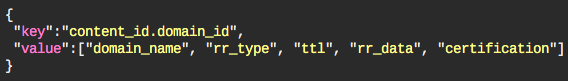
\includegraphics[scale=0.5]{figure/content-file.png}
 \caption{コンテンツファイルのデータフォーマット}
 \label{fig:manager-provider}
\end{figure}

\subsection{動作メカニズム}
\subsubsection{レコード情報に対する操作}
本項では,SORESにおいて使用されるリソースレコードのタイプと
%TTLの更新方法について説明する

\subsubsection{名前解決}
%ハッシュテーブルのレプリケーション手法
%特定のハッシュ範囲を管理するノードは,複数用意させ,そのアドレスを対応表に明記し,ストアする際にその全てのレプリケーションサーバにストアリクエストする
%イベントドリブン
%非同期
